\documentclass{article}
\usepackage{tikz}

\begin{document}

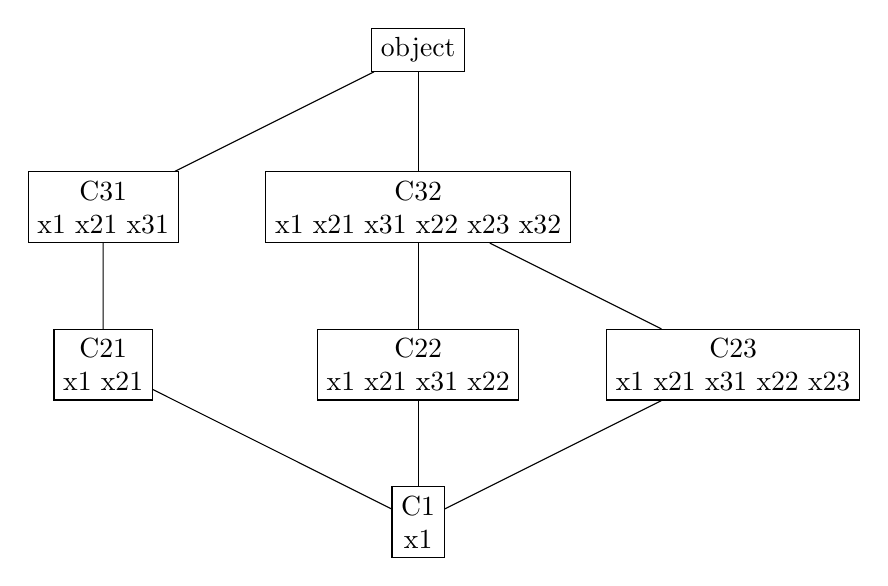
\begin{tikzpicture}[align=center]
\node[draw] (O) at (4, 6) {object};
\node[draw] (C31) at (0, 4) {C31\\x1 x21 x31};
\node[draw] (C32) at (4, 4) {C32\\x1 x21 x31 x22 x23 x32};
\node[draw] (C21) at (0, 2) {C21\\x1 x21};
\node[draw] (C22) at (4, 2) {C22\\x1 x21 x31 x22};
\node[draw] (C23) at (8, 2) {C23\\x1 x21 x31 x22 x23};
\node[draw] (C1) at (4, 0) {C1\\x1};
\draw (O) -- (C31);
\draw (O) -- (C32);
\draw (C31) -- (C21) -- (C1); 
\draw (C32) -- (C22) -- (C1); 
\draw (C32) -- (C23) -- (C1); 

\end{tikzpicture}
\end{document}  